\documentclass[11pt]{article}\usepackage[]{graphicx}\usepackage[]{color}
%% maxwidth is the original width if it is less than linewidth
%% otherwise use linewidth (to make sure the graphics do not exceed the margin)
\makeatletter
\def\maxwidth{ %
  \ifdim\Gin@nat@width>\linewidth
    \linewidth
  \else
    \Gin@nat@width
  \fi
}
\makeatother

\definecolor{fgcolor}{rgb}{0.345, 0.345, 0.345}
\newcommand{\hlnum}[1]{\textcolor[rgb]{0.686,0.059,0.569}{#1}}%
\newcommand{\hlstr}[1]{\textcolor[rgb]{0.192,0.494,0.8}{#1}}%
\newcommand{\hlcom}[1]{\textcolor[rgb]{0.678,0.584,0.686}{\textit{#1}}}%
\newcommand{\hlopt}[1]{\textcolor[rgb]{0,0,0}{#1}}%
\newcommand{\hlstd}[1]{\textcolor[rgb]{0.345,0.345,0.345}{#1}}%
\newcommand{\hlkwa}[1]{\textcolor[rgb]{0.161,0.373,0.58}{\textbf{#1}}}%
\newcommand{\hlkwb}[1]{\textcolor[rgb]{0.69,0.353,0.396}{#1}}%
\newcommand{\hlkwc}[1]{\textcolor[rgb]{0.333,0.667,0.333}{#1}}%
\newcommand{\hlkwd}[1]{\textcolor[rgb]{0.737,0.353,0.396}{\textbf{#1}}}%

\usepackage{framed}
\makeatletter
\newenvironment{kframe}{%
 \def\at@end@of@kframe{}%
 \ifinner\ifhmode%
  \def\at@end@of@kframe{\end{minipage}}%
  \begin{minipage}{\columnwidth}%
 \fi\fi%
 \def\FrameCommand##1{\hskip\@totalleftmargin \hskip-\fboxsep
 \colorbox{shadecolor}{##1}\hskip-\fboxsep
     % There is no \\@totalrightmargin, so:
     \hskip-\linewidth \hskip-\@totalleftmargin \hskip\columnwidth}%
 \MakeFramed {\advance\hsize-\width
   \@totalleftmargin\z@ \linewidth\hsize
   \@setminipage}}%
 {\par\unskip\endMakeFramed%
 \at@end@of@kframe}
\makeatother

\definecolor{shadecolor}{rgb}{.97, .97, .97}
\definecolor{messagecolor}{rgb}{0, 0, 0}
\definecolor{warningcolor}{rgb}{1, 0, 1}
\definecolor{errorcolor}{rgb}{1, 0, 0}
\newenvironment{knitrout}{}{} % an empty environment to be redefined in TeX

\usepackage{alltt}
\title{Lab 2 - Linguistic Data\\
  Stat 215A, Fall 2015}
\author{Diego Ponce De Leon Barido, Katerina Georgiou, Kellie Ottoboni, Steve Howard}

\usepackage{amsmath,amssymb,amsthm}
\usepackage{graphicx,float}
\usepackage[margin=0.75in]{geometry}
\usepackage{bm}
\setlength{\parskip}{\medskipamount}
\setlength{\parindent}{0cm}
\usepackage{subcaption}
\IfFileExists{upquote.sty}{\usepackage{upquote}}{}
\begin{document}






% latex table generated in R 3.2.2 by xtable 1.7-4 package
% Sat Oct 17 18:03:40 2015
\begin{table}[ht]
\centering
\begin{tabular}{rlll}
  \hline
 & N.Days & First Date & Last Date \\ 
  \hline
E.Fridge & 15 & 2015-07-14 & 2015-07-29 \\ 
  Inside Temp & 15 & 2015-07-14 & 2015-07-29 \\ 
  E.House & 15 & 2015-07-14 & 2015-07-29 \\ 
  Ambient & 15 & 2015-07-14 & 2015-07-29 \\ 
   \hline
\end{tabular}
\end{table}






\begin{knitrout}
\definecolor{shadecolor}{rgb}{0.969, 0.969, 0.969}\color{fgcolor}

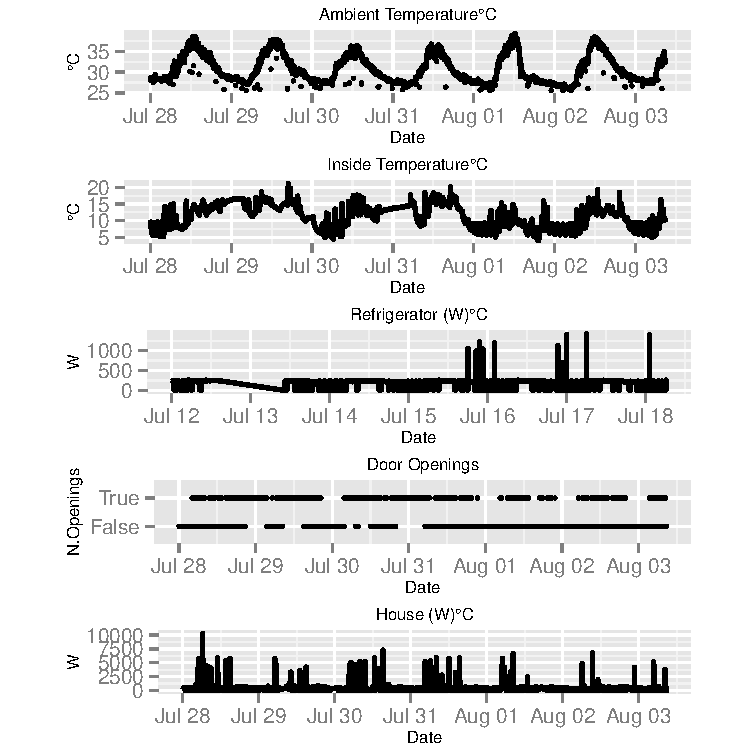
\includegraphics[width=\maxwidth]{figure/timeseriesplotsetup-1} \hfill{}



\end{knitrout}


\begin{knitrout}
\definecolor{shadecolor}{rgb}{0.969, 0.969, 0.969}\color{fgcolor}

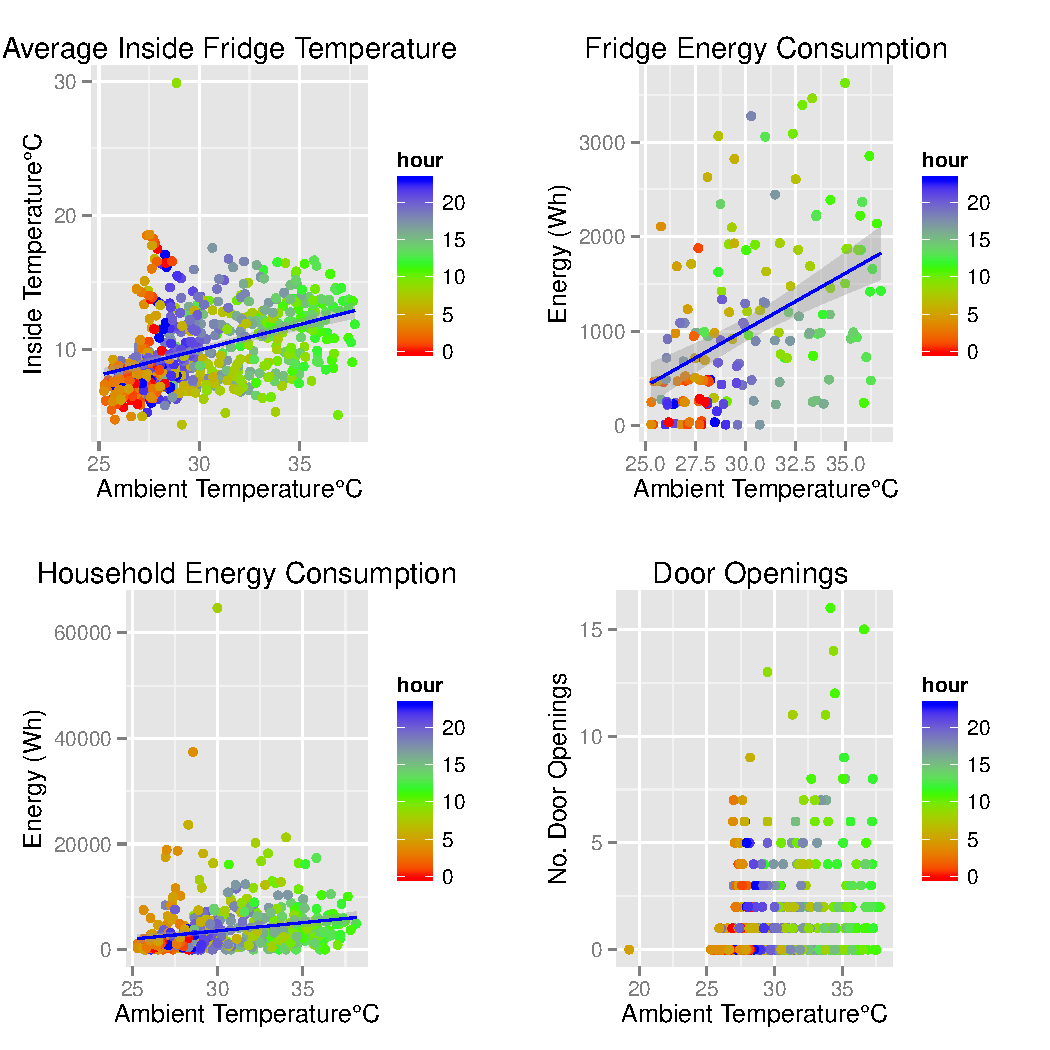
\includegraphics[width=\maxwidth]{figure/correlationplots-1} \hfill{}



\end{knitrout}
    
      










\end{document}

